\clearpage

\subsection{例題10 シューティングゲームの絵を改造する}

\subsubsection*{考え方}

シューティングゲーム(shoot.hsp)の絵を改造して自分だけの絵にしてみましょう。
シューティングゲームの絵は、「/home/ユーザー名/02/chr.png」というファイルに保存されています。
改造ができたらTAや周りの友達にも見せてあげましょう。

\subsubsection*{例題10 答え}

教科書でドロップパズルの絵を修正したのと同じように、GIMPを使ってシューティングゲームの絵を修正します。

ファイルマネージャーの画面から、「/home/ユーザー名/02」フォルダにある「chr.png」のアイコンで右クリックを押して、「GIMP ( GNU Image Manipulation Program )」のメニューを選ぶすることでツールを起動させることができます。
これで、「chr.png」を読み込んで下絵とすることができます。

\begin{figure}[H]
    \begin{center}
        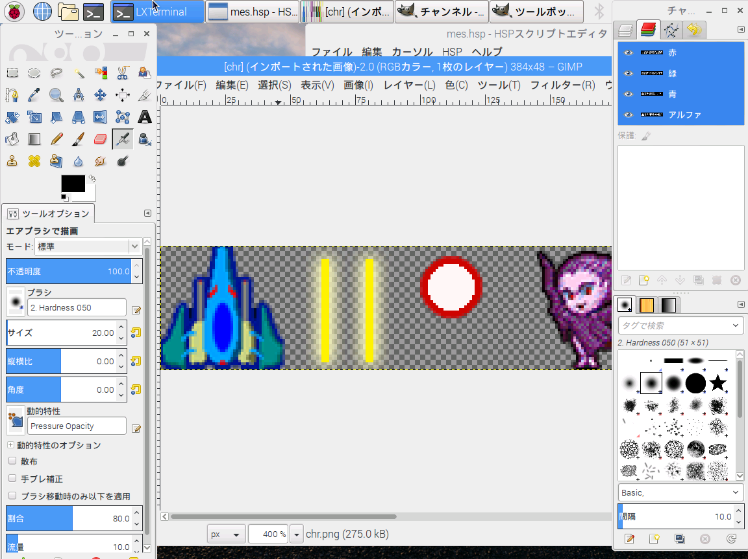
\includegraphics[keepaspectratio,width=8.625cm,height=6.459cm]{text02-img/text02-img042.png}
        \caption{chr.pngを読み込んだ画面}
    \end{center}
\end{figure}

左にあるのが自機、その右にあるのがレーザー、その右は敵の弾です。ゲームのキャラクターを改造してみましょう。
作業が終わったら、ファイル→「chr.pngに上書きエクスポート」を選んで保存します。

時間のある人は、他の絵の書き換えにも挑戦してみましょう。
背景は「bg.png」、キャラクターは「chr.png」、タイトルは「title.png」です。

※もし、chr.png の内容を元に戻したい時には、/usr/local/share/ome/02/chr.png のファイルを /home/ユーザー名/02 フォルダに上書きでコピーすれば元に戻せます。

GIMPを使い終わったら、最後にファイル→「終了」を選んでGIMPアプリケーションを閉じてください。

